\documentclass[11pt]{article} % 
\usepackage[pdftex]{graphicx}
\usepackage{fullpage}
\usepackage{graphicx}
\usepackage{graphics}
\usepackage{psfrag}
\usepackage{pgf}
\usepackage{color}
\usepackage{tikz}
\usetikzlibrary{arrows,automata}
\usepackage[latin1]{inputenc}
\usepackage{amsthm}
\usepackage{amsmath,amssymb}
\usepackage{enumerate}
\setlength{\textwidth}{6.5in}
\setlength{\textheight}{9in}
\newcommand{\N}{\mathbb{N}}
\newcommand{\Z}{\mathbb{Z}}
\newcommand{\R}{\mathbb{R}}
\newcommand{\Q}{\mathbb{Q}}
\newcommand{\C}{\mathbb{C}}
\newcommand{\PP}{\mathbb{P}}
\newcommand{\tab}{\;\;\;\;\;}
\newcommand{\inv}{^{-1}}
\newcommand{\tr}{\textrm}
\newcommand{\lc}{\sqcup}
\newcommand{\var}{\tr{Var}}
\newcommand{\cov}{\tr{Cov}}
\newcommand{\like}{\mathcal{L}}

\begin{document}

\hfill Robert Johns

\hfill February 13, 2014

\begin{center} {\Large CSCI 678: Statistical Analysis of Simulation Models}\\{\large Homework 4}\end{center}

\begin{enumerate}

%1
\item Given that $X_1, X_2, \ldots, X_n$ are iid exponential random variables with mean $\alpha$, show that $Y = \frac{2}{\alpha}\sum_{i = 1}^n X_i$ is Chi-square with $2n$ degrees of freedom.

{\bf Solution:} Using the MGF technique, we have
\begin{align*}
M_Y(t) &= E[e^{tY}]\\
&= E[e^{(2t/\alpha)\sum_{i = 1}^nX_i}]\\
&= E[e^{t(\sum_{i =1}^n2X_i/\alpha)}]\\
&= E[e^{t\cdot2X_1/\alpha}e^{t\cdot2X_2/\alpha}\cdots e^{t\cdot2X_n/\alpha}]\\
&= E[e^{t\cdot2X_1/\alpha}]E[e^{t\cdot2X_2/\alpha}]\cdots E[e^{t\cdot2X_n/\alpha}]\\
&= M_{X_1}(2t/\alpha)M_{X_2}(2t/\alpha)\cdots M_{X_n}(2t/\alpha)\\
&= (1-2t)\inv(1-2t)\inv\cdots(1-2t)\inv\\
&= (1-2t)^{-n} & t < 1/2
\end{align*}

which is the MGF for a $\chi^2(2n)$ random variable.

%%%%%
%2
\item Verify the two nonlinear equations on page 286 in Law for the MLE's corresponding to the Weibull distribution.  These equations are
\begin{align*}\frac{\sum_{i = 1}^nx_i^\alpha \ln(x_i)}{\sum_{i = 1}^n x_i^\alpha} - \frac{1}{\alpha} = \frac{\sum_{i = 1}^n \ln(x_i)}{n}
&\tr{\hspace{1 cm}and\hspace{1 cm}}
\beta = \left(\frac{\sum_{i = 1}^nx_i^\alpha}{n}\right)^{1/\alpha}\end{align*}

{\bf Solution:} The likelihood function for the Weibull distribution is:
$$\like(\alpha, \beta \;|\;x) = \alpha\beta^{-\alpha}x^{\alpha -1}e^{-(x/\beta)^\alpha}$$

Taking the natural logarithm, we get:

$$\ln [\like(\alpha, \beta \;|\;x)] = \ln(\alpha) - \left(\frac{x}{\beta}\right)^\alpha - \alpha\ln(\beta) + (\alpha - 1)\ln(x)$$

We then take the partial derivatives with respect to $\alpha$ and $\beta$ to get:

$$\frac{\partial\ln\like}{\partial\alpha} = \frac{1}{\alpha} + \left(\frac{x}{\beta}\right)^\alpha\left[-\ln\left(\frac{x}{\beta}\right)\right] - \ln(\beta) + \ln(x)$$

$$\frac{\partial\ln\like}{\partial\beta} = \frac{\alpha\left[\left(\frac{x}{\beta}\right)^\alpha - 1\right]}{\beta}$$

Then, we assume that we have many random variates, set that sum equal to 0 and use the fact that the derivative of the sum is the sum of the derivatives to get 

\begin{align*}
\frac{\partial\ln\like_{(n)}}{\partial\beta} = 0 &= \sum_{i = 1}^n \frac{\alpha\left[\left(\frac{x_i}{\beta}\right)^\alpha - 1\right]}{\beta}\\
0&= \frac{\alpha}{\beta^{\alpha+1}}\sum_{i = 1}^nx_i^\alpha - \frac{n\alpha}{\beta}\\
\frac{n\alpha}{\beta} &= \frac{\alpha}{\beta^{\alpha+1}}\sum_{i = 1}^nx_i^\alpha\\
\beta &= \left(\frac{\sum_{i = 1}^nx_i^\alpha}{n}\right)^{\frac{1}{\alpha}}
\end{align*}

and

\begin{align*}
\frac{\partial\ln\like_(n)}{\partial\alpha} = 0 & = \sum_{i = 1}^n\left(\frac{1}{\alpha} + \left(\frac{x_i}{\beta}\right)^\alpha\left[-\ln\left(\frac{x}{\beta}\right)\right] - \ln(\beta) + \ln(x)\right)\\
0 &= \frac{n}{\alpha} - \frac{1}{\beta^\alpha}\sum_{i = 1}^nx_i^\alpha\left[\ln\left(\frac{x^i}{\beta}\right)\right] - n\ln(\beta) + \sum_{i = 1}^n\ln(x_i)\\
0 &= \frac{n}{\alpha} - n\ln(\beta) + \sum_{i = 1}^n\ln(x_i) - \beta^{-\alpha}\sum_{i = 1}^nx_i^\alpha\ln(x_i) + \beta^{-\alpha}\ln(\beta)\sum_{i = 1}^nx_i^{\alpha}
\end{align*}
$$0 = \frac{n}{\alpha} - n\ln\left(\left(\frac{\sum_{i = 1}^nx_i^\alpha}{n}\right)^{\frac{1}{\alpha}}\right) + \sum_{i = 1}^n\ln(x_i) - \left(\left(\frac{\sum_{i = 1}^nx_i^\alpha}{n}\right)^{\frac{1}{\alpha}}\right)^{-\alpha}\sum_{i = 1}^nx_i^\alpha\ln(x_i) +$$
$$\left(\left(\frac{\sum_{i = 1}^nx_i^\alpha}{n}\right)^{\frac{1}{\alpha}}\right)^{-\alpha}\ln\left(\left(\frac{\sum_{i = 1}^nx_i^\alpha}{n}\right)^{\frac{1}{\alpha}}\right)\sum_{i = 1}^nx_i^{\alpha}$$

which is the nastiest equation I have ever seen.  But after a little wailing and gnashing of teeth, we end up with: 

$$\frac{\sum_{i = 1}^nx_i^\alpha \ln(x_i)}{\sum_{i = 1}^n x_i^\alpha} - \frac{1}{\alpha} = \frac{\sum_{i = 1}^n \ln(x_i)}{n}$$

which is the equation we are looking for.

\newpage
%%%%%
%3
\item$\\$\begin{figure}[ht]
\begin{minipage}[b]{0.45\linewidth}
\centering
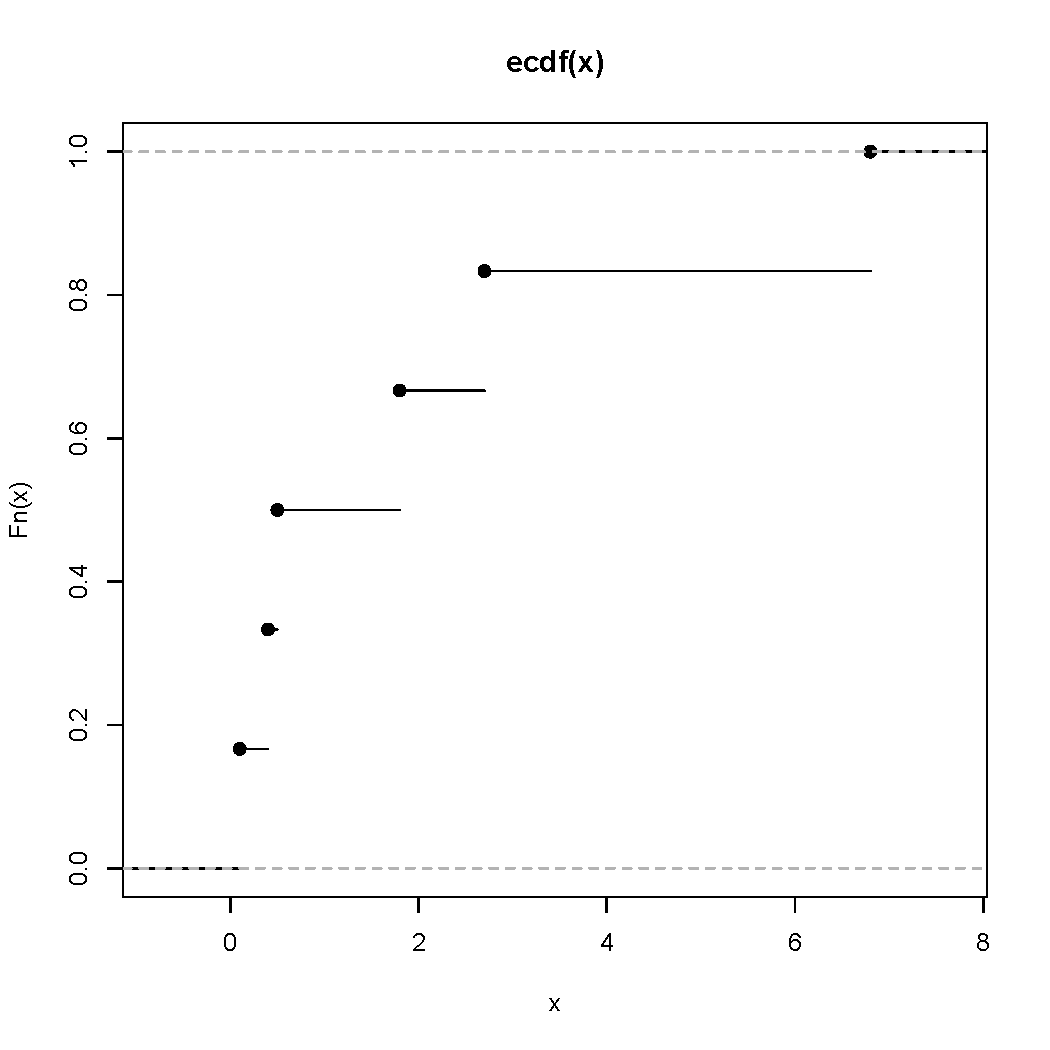
\includegraphics[width=6cm]{ecdf1.pdf}
\caption{(a)}
\label{fig:figure1}
\end{minipage}
\hspace{0.5cm}
\begin{minipage}[b]{0.45\linewidth}
\centering
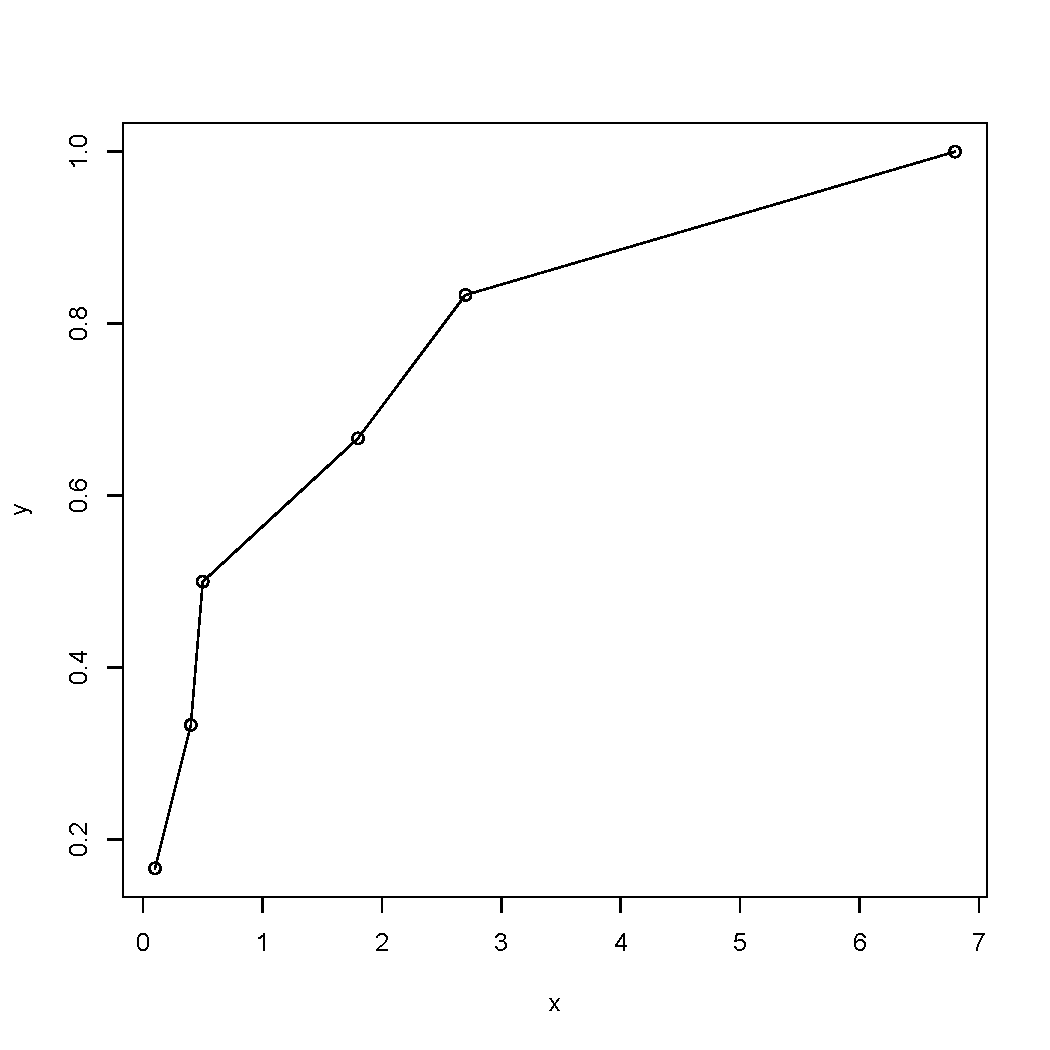
\includegraphics[width=6cm]{ecdf2.pdf}
\caption{(b)}
\label{fig:figure2}
\end{minipage}
\end{figure}

\begin{figure}[ht]
\begin{minipage}[b]{0.45\linewidth}
\centering
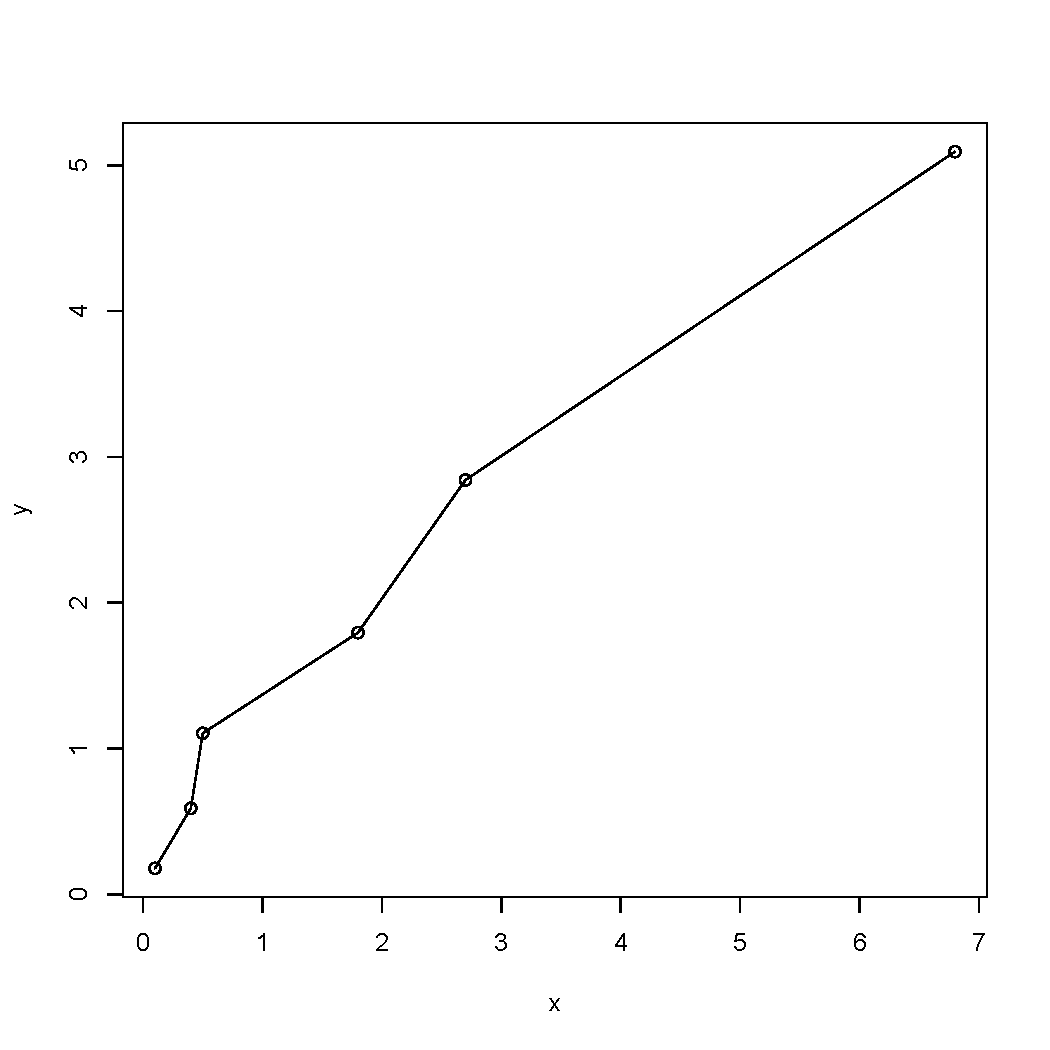
\includegraphics[width=6cm]{asm3e.pdf}
\caption{(e)}
\label{fig:figure1}
\end{minipage}
\hspace{0.5cm}
\begin{minipage}[b]{0.45\linewidth}
\centering
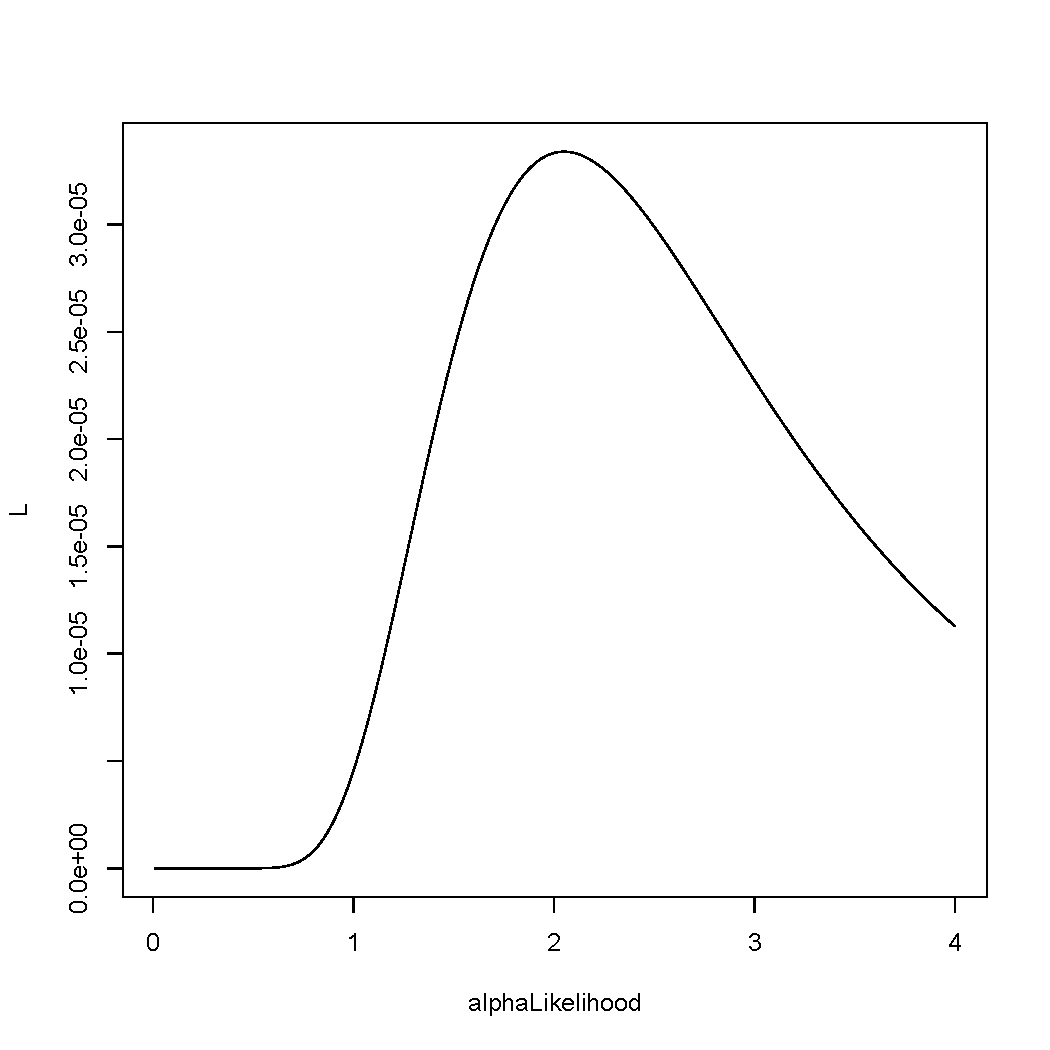
\includegraphics[width=6cm]{asm3f.pdf}
\caption{(f)}
\label{fig:figure2}
\end{minipage}
\end{figure}

\begin{enumerate}

%3c
\setcounter{enumii}{2}
\item mean: 2.05, variance: 6.395, skewness: 0.946086, kurtosis: 2.188036, coefficient of variation: 1.233577 

%3d
\item The likelihood function for the exponential distribution is 
$$L(\alpha) = \prod_{i=1}^6 \frac{1}{\alpha}e^{-x_i/\alpha}$$ 
so taking the natural logarithm, we see that the log-likelihood function is 
$$\ln L = \sum_{i=1}^6\left(-\ln(\alpha)-\frac{x_i}{\alpha}\right)$$
which simplifies to 
$$\ln L = -6\ln(\alpha) - \frac{1}{\alpha}\sum_{i=1}^6 x_i = -6\ln(\alpha) - \frac{6\overline{x}}{\alpha}$$ 
So
$$\frac{\partial \ln L}{\partial \alpha} = -\frac{6}{\alpha} + \frac{6\overline{x}}{\alpha^2}=0$$
which, when given to a computer that is smarter than I am, yields $\hat{\alpha} = \overline{x} = 2.05$.

%3g
\setcounter{enumii}{6}
\item We have this equation for the confidence interval:

$$\frac{2\sum_{i = 1}^6x_i}{\chi^2_{12, 1 - .95/2}} < \hat{\alpha} < \frac{2\sum_{i = 1}^6x_i}{\chi^2_{12, .95/2}}$$

Using the result from (1), we have

$$\frac{24.6}{23.33666} < \hat{\alpha} < \frac{24/6}{4.403789}$$
so our confidence interval is:
$$1.054 < \hat{\alpha} < 5.586$$

%3h
\item The program \texttt{asm3h.r} was used to calculate the value.  the output is as follows:
\begin{verbatim}[1] "critical value:"
[1] 1.094
[1] "adjusted test statistic:"
[1] 0.7290758\end{verbatim}

Since the test statistic is lower than the critical value, this supports the statement that the data came from an exponential population distribution with significance .05.

\end{enumerate}

%%%%%
%4
\item See attached code (\texttt{asm4b.c}).  We see from the output that when the arrivals are one exponential random variable, the average wait is 3.802564, and when the arrivals are the average of three exponentials, the average wait is 2.153414.  Let's examine why this could be true.  Because the mean wait time decreased, and the only factor we changed is the arrival time, the arrival time must be affecting the wait time.  Logically, there's an inverse relationship between the interarrival time and the wait time (if it takes longer for people to arrive, the system has less to deal with and so moves people throughout faster).  So these numbers make sense, because due to the shape of an exponential distribution, if we average three random variates, theres a bigger chance that one of them will be far enough to the right to throw off the other two than there is that one variate is very far to the right.

%%%%%
%5
\item R code gives us the following results:
\begin{verbatim}   1.6515497424
x1 0.0002241861
x2 4.0807366362\end{verbatim}

The top number is the intercept, $\hat{\alpha}$. The variable $x1$ is the regression coefficient of population vs crime rate and $x2$ is the regression coefficient of illiteracy rate vs crime rate.  We see that $x1$ is basically 0, so there is little (though slightly positive) correlation between population size and crime rate.  However, there is a much larger regression coefficient between illiteracy rate and crime rate, implying that people who can't read steal things.

\end{enumerate}

\end{document}